%; whizzy chapter
% -initex iniptex -latex platex -format platex -bibtex jbibtex -fmt fmt
% 以上 whizzytex を使用する場合の設定。

%     Kansai Debian Meeting resources
%     Copyright (C) 2007 Takaya Yamashita
%     Thank you for Tokyo Debian Meeting resources

%     This program is free software; you can redistribute it and/or modify
%     it under the terms of the GNU General Public License as published by
%     the Free Software Foundation; either version 2 of the License, or
%     (at your option) any later version.

%     This program is distributed in the hope that it will be useful,
%     but WITHOUT ANY WARRANTY; without even the implied warranty of
%     MERCHANTABILITY or FITNESS FOR A PARTICULAR PURPOSE.  See the
%     GNU General Public License for more details.

%     You should have received a copy of the GNU General Public License
%     along with this program; if not, write to the Free Software
%     Foundation, Inc., 51 Franklin St, Fifth Floor, Boston, MA  02110-1301 USA

%  preview (shell-command (concat "evince " (replace-regexp-in-string "tex$" "pdf"(buffer-file-name)) "&"))
% 画像ファイルを処理するためにはebbを利用してboundingboxを作成。
%(shell-command "cd image200708; ebb *.png")

%%ここからヘッダ開始。

\documentclass[mingoth,a4paper]{jsarticle}
\usepackage{kansaimonthlyreport}
\usepackage[dvips]{xy}
\usepackage{ascmac}

% 日付を定義する、毎月変わります。
\newcommand{\debmtgyear}{2010}
\newcommand{\debmtgdate}{24}
\newcommand{\debmtgmonth}{10}
\newcommand{\debmtgnumber}{40}

\begin{document}

\begin{titlepage}

% 毎月変更する部分、本文の末尾も修正することをわすれずに

 第\debmtgnumber{}回 関西 Debian 勉強会資料

\vspace{2cm}

\begin{center}
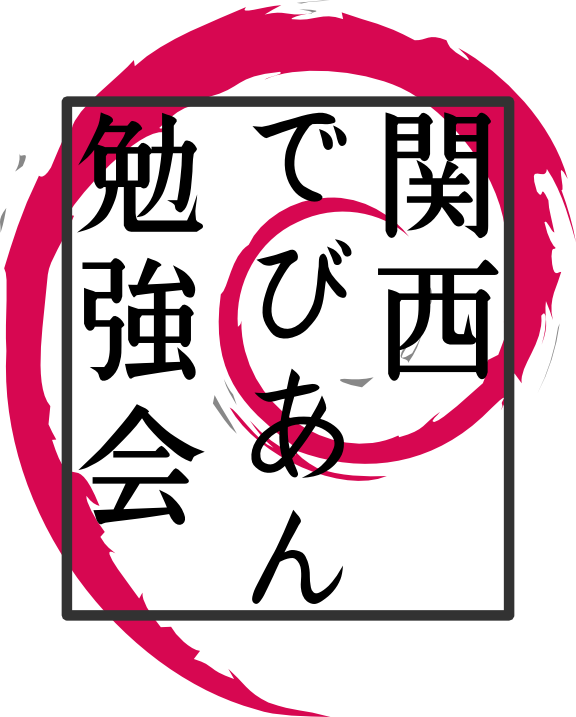
\includegraphics{image200802/kansaidebianlogo.png}
\end{center}

\begin{flushright}
\hfill{}関西 Debian 勉強会担当者 佐々木・倉敷・のがた \\
\hfill{}\debmtgyear{}年\debmtgmonth{}月\debmtgdate{}日
\end{flushright}

\thispagestyle{empty}
\end{titlepage}

\dancersection{Introduction}{Debian JP}

\subsection*{}%ロゴ用のスペース稼ぎ

関西 Debian 勉強会はDebian GNU/Linux のさまざまなトピック(新しいパッケー
ジ、Debian 特有の機能の仕組、Debian 界隈で起こった出来事、などなど)に
ついて話し合う会です。

目的として次の三つを考えています。
\begin{itemize}
      \item MLや掲示板ではなく、直接顔を合わせる事での情報交換の促進
      \item 定期的に集まれる場所
      \item 資料の作成
\end{itemize}

それでは、楽しい一時をお楽しみ下さい。

\clearpage

\begin{minipage}[b]{0.2\hsize}
 {\rotatebox{90}{\fontsize{80}{80}
{\gt 関西 Debian 勉強会}}}
\end{minipage}
\begin{minipage}[b]{0.8\hsize}
\hrule
\vspace{2mm}
\hrule
\setcounter{tocdepth}{1}
\tableofcontents
\vspace{2mm}
\hrule
\end{minipage}

\dancersection{最近のDebian関係のイベント報告}{Debian JP}

\subsection{第 39 回関西 Debian 勉強会}

前回の関西 Debian 勉強会は、9 月 26 日に
(財)京都高度技術研究所(ASTEM)\footnote{\url{http://www.astem.or.jp/}}様のご協力のもと
「タイル型ウィンドウマネージャ対決」という内容で行なわれました。
%
山田洋平さんによるタイル型ウィンドウマネージャの入門と dwm の解説、
倉敷悟さんによる xmonad の解説、
山下尊也さん(久々参加!!)による awesome の解説が非常に濃ゆく行なわれました
のがたさんによる
「この濃さなら、
資料書いてもらうべきだっだんじゃね?(by nogajun)」という呟きもありましたが
%
参加者も皆さん楽しんで頂けたのではないでしょうか?

勉強会後は同じ会場でビアバッシュ、ということで、ピザとビールで歓談しました。
ちなみにその場で KOF のタイトルが決まったりしました。
以前やまねさんに言われました通り、
関西は毎度毎度飲み会で物事が決まるみたいです(笑)。


\subsection{2010 年度日本 OSS 貢献者賞・日本 OSS 奨励賞}

IPA より 2010 年度日本 OSS 貢献者賞・日本 OSS 奨励賞受賞者の発表がありました%
\footnote{\url{http://www.ipa.go.jp/about/press/20101015_2.html}}。
今年度は Debian JP Project より、
武藤 健志さんが OSS 貢献者賞、岩松 信洋さんが OSS 奨励賞を受賞しました。
素晴しいですね。

\subsection{第 69 回東京エリア Debian 勉強会}

10 月 16 日に東京エリアDebian勉強会が開かれました。
特集として「俺の Debian な一日」という事前課題が報告されています。
非常に興味深いので、一度ご覧下さい%
\footnote{%
\url{http://tokyodebian.alioth.debian.org/pdf/debianmeetingresume201010.pdf}}
\footnote{個人的には、小室文さんの生活がうらやましすぎる...}.
セッションは OSC 北海道の報告、
Debconf10 の報告、上川さんによる「俺の Debian な一日」でした。

また Debian Miniconf in Japan に関するブレストが行なわれています。

日本で Debconf を開催する/日本に誘致するために、
先ずは Miniconf の開催から始めよう、という計画です。
興味のある方は、勉強会資料をご覧下さい。
また、ご意見ある方は隔週木曜に開催されている
IRC ミーティングへ参加してみては如何でしょうか?
\footnote{%
IRC サーバ: {\tt{irc.debian.or.jp:6667}}、
チャンネルは {\tt{\#debianjp}}、文字コード: UTF-8 です。}

\dancersection{事前課題}{Debian JP}

今回は以下の課題を設定しました。
%
\begin{quote}
    \begin{screen}
         レスキュー用途とインストール用途を除く、
        ライブシステムを使用する状況や用途を教えて(または考えて)ください。
    \end{screen}
\end{quote}
%
参加者の皆さんによる回答は以下の通りです。

\begin{prework}{ Ipv6waterstar }

現在, インストールしている Debian システムの環境を変えずに別のシステム環境を試したい時など.

\end{prework}



\begin{prework}{ dictoss (杉本  典充) }

    \begin{itemize}
          \item 公共スペースに設置するパソコンのブートディスクとして使用する.
         \\
        そうすると OS やアプリの設定を勝手に変えられても再起動すれば直るため, OS の修復の手間が省ける.
        (ネットワークブートという手もあるが, ライブシステムはスタンドアロンで起動可能な分, 敷居が低い)
\end{itemize}

\end{prework}



\begin{prework}{ 山田 洋平 }

昔 1FD Linux で HDD の載ってない古い PC を動かして, 起動後はディスクレスだから静穏とか言ってました. ルータとかに使ってました. そういうのとか.
あるいはいろんな環境をとっかえひっかえ試すとか. ソフトのテスト環境としてとか. (仮想化でもいいのだけど)

\end{prework}



\begin{prework}{ かわだてつたろう }

    \begin{itemize}
          \item 借り物の PC や不特定の人が使う PC で自分好みの環境を使うため
          \item 複数の人に同じ環境, アプリケーションを使ってもらいたい場合.
        「第 37 回関西 Debian 勉強会@OSC2010 Kyoto 」とか OSM で JOSM の使い方講習をするといったような用途
    \end{itemize}


\end{prework}



\begin{prework}{ 八津尾  雄介 }
    \begin{enumerate}
          \item パーティションが一杯になって拡張が必要なとき.
        (これもレスキューですか?)
          \item 自分の環境を持ち歩きたいとき.
    \end{enumerate}

\end{prework}



\begin{prework}{@tetsu\_koba }

例えば, 同僚が「今日は一日外出するのでデスクトップ PC は使わない」とする.
その PC をライブ CD で起動して distcc のサーバを動かす.
ビルドする時にその PC の CPU パワーを借りて分散コンパイルする.

これがお手軽にできるセットがあったら使ってみたい.

\end{prework}



\begin{prework}{ 山下康成 }

藤丸君のように, USB メモリでいつでも自分のハッキング環境が持ち歩けるのではないでしょうか

\end{prework}



\begin{prework}{ 佐藤誠 }

    \begin{itemize}
          \item データ削除 \\
        wipe-out のように, それに特化したライブシステムもあります.
          \item アドホックなシステム構築 \\
常時接続の切れたとき, 即席のルータを構築して凌いだことがあります.
このような時は, ユーザデータや余計な設定のないライブシステムが便利だと思います.
Knoppix Hacks には, MySQL データベースの即席構築例が載っていました
(まあ, このあたりもレスキュー用途に入りそうですが)
    \end{itemize}

\end{prework}



\begin{prework}{ 西山和広 }

    uuuu という勉強会\footnote{\url{http://www.cuzic.com/undefineduniversityuponustream}}
    で YouTube の講義ビデオを再生するのに, ノート PC の内蔵 HDD が不調のため, netboot のライブ環境を使っています.
    プログラムのテスト環境にも使いたいのですが, データベースを使うものの場合, メモリ不足で厳しいようです.

\end{prework}



\begin{prework}{ "まさ"こと"甲斐正三"です }

以下の用途は実施したことはありませんが, 実施可能性ありと
思われる場面を想定したものです.
\begin{itemize}
      \item 教育用途 (案) \\
    セミナーのハンズオンを行うとき, 受講者全員に共通な環境を提供する.
      \item 新規システム等の評価検討用 (案) \\
    新規システムや新規ソフトウエアを事前評価,
    検討する際に使用する.
    例として,
    \begin{itemize}
          \item ある PC に Debian をインストールできそうかどうかをその PC 自体を使って Live CD で起動してみる.
    \end{itemize}
\end{itemize}

\end{prework}



\begin{prework}{ takuya.1st }

シンクライアントとか?

みんなが帰ったとの PC にライブシステム突っ込んで分散処理を作るとか?

もちろん, ソフトウェアのデモ用にも使えますよね.
KOF のような展示会用に PC を毎回作らなくても CD 用意して持って行けば OK とか


\end{prework}



\begin{prework}{ lurdan }

最近は起動も速いみたいだし, なんらかのクラウドストレージを HOME として組み込んだら, シンプルなクライアントとしては充分だったりするんじゃないかと妄想.

\end{prework}



\begin{prework}{ 佐々木洋平 }

以前, ハンズオン形式の実習/ 教育機関での計算機演習などで, 受講者の環境を揃えるために使用しました (その時には, CentOS と Debian の dual boot な環境が必要で, DebianLive のエキスパートであるのがたさんに助けて頂きました).

\end{prework}



\begin{prework}{ のがたじゅん }

古くなった PC にライブシステムを組み込みメンテナンスフリーなシステムを作りました. ほかにはネットワークからブートするライブシステムで面白いことできないかなーと思案中.

\end{prework}




\dancersection{initramfs について}{西山 和広}
\subsection{initrd/initramfs とは?}

\begin{itemize}
\item Linux の起動途中に使われる root ファイルシステム
\item この中で本当の root ファイルシステム (real root) をマウント
\item 実体は gzip された cpio アーカイブ

\begin{itemize}
\item 昔は ext2 のディスクイメージファイル
\item gzip の代わりに lzma のこともある (casper/initrd.lz など)
\end{itemize}

\end{itemize}
\subsection{いろいろなところからの Linux の起動}

\subsubsection{USB/HDD から起動}

\begin{itemize}
\item BIOS (起動順位で USB/HDD が上)
\item MBR (grub などのブートローダー)
\item vmlinuz (カーネル) + initrd (の中の /init)
\item real root (/dev/sda1 とか) の /sbin/init
    (MD, LVM2, LUKS などでも OK)
\item /etc/inittab の処理とか
\end{itemize}
\subsubsection{光学ドライブから起動}

\begin{itemize}
\item BIOS (起動順位で光学ドライブが上)
\item El Torito (isolinux などのブートローダー)
\item vmlinuz (カーネル) + initrd (の中の /init)
\item real root (filesystem.squashfs + aufs とか) の /sbin/init
\item /etc/inittab の処理とか
\end{itemize}
\subsubsection{ネットワークから起動}

\begin{itemize}
\item BIOS (起動順位で NIC が上)
\item PXE boot (pxelinux などのブートローダー)
\item vmlinuz (カーネル) + initrd (の中の /init)
\item real root (NFS とか) の /sbin/init
\item /etc/inittab の処理とか
\end{itemize}
\subsubsection{real root の場所}

  カーネルに root=UUID=xxx などで指定
\begin{itemize}
\item ローカルディスク (root=/dev/sda1 など)
\item 光学ドライブ (root=/dev/hdc など)
\item NFS (nfsroot=192.168.0.1:/path/to/nfsroot など)
\end{itemize}
  など

\subsubsection{/proc/cmdline}

\begin{itemize}
\item カーネルのコマンドライン引数
\item カーネルパラメーター
\item 起動後に /proc/cmdline で見えるもの
\item grub などで vmlinuz の後ろに書いているもの
\item initramfs の処理で使うものが多い
\item カーネル自体が処理するものもある
\item real root で起動するプログラムが参照する目的で使っても良いが、カーネルや initramfs が使うものと衝突しないように注意
\end{itemize}
\subsubsection{/proc/cmdline で良く使われるものの例}

\begin{description}
      \item [quiet]  \\起動中のコンソールへの出力を減らす
      \item [ro / rw]  \\ initramfs の中で real root を readonly mount するかどうか
      \item [\texttt{init=/path/to/real\_init}]  \\/sbin/init の代わりに実行するプログラムを指定
      \item [acpi=off apm=off など]  \\カーネルが処理
      \item [text]  \\ /etc/init.d/gdm3 が「grep -wqs text /proc/cmdline」でチェックしている
      \item [root=/path/to/blockdevice]  \\ ルートファイルシステムとしてマウントするデバイスを指定
      \item [boot=local / boot=nfs / boot=casper / boot=live]  \\real root を mount するのに使うスクリプトを指定
\end{description}
\subsection{initramfs について}

\subsubsection{update-initramfs}

\begin{itemize}
\item initramfs はパッケージの中身ではない
\item update-initramfs コマンドで生成や更新
    (カーネルのパッケージのインストール時などは dpkg-trigger で遅延実行)
\item \texttt{/usr/share/initramfs-tools/} や \texttt{/etc/initramfs-tools/} を元に生成
\item 「sudo update-initramfs -u -k all」などで更新
\end{itemize}
\subsubsection{initramfs の調べ方}
\begin{commandline}
 mkdir -p /tmp/initrd && (cd /tmp/initrd && { zcat /boot/initrd.img-* | cpio -idm; })
 # initramfs-tools(8)
 mkdir tmp/initramfs
 cd tmp/initramfs
 gunzip -c /boot/initrd.img-2.6.18-1-686 | \
 cpio -i -d -H newc --no-absolute-filenames
 # linux-2.6/Documentation/initrd.txt
 mkdir /tmp/imagefile
 cd /tmp/imagefile
 gzip -cd /boot/imagefile.img | cpio -imd --quiet
\end{commandline}

などのように展開
(カレントディレクトリにばらまかれるので展開場所には注意)

\subsubsection{initramfs の中身}

\begin{description}
\item [./init]  \\
カーネルが実行するプログラム
\begin{itemize}
      \item Debian 系の場合は /bin/sh のシェルスクリプト
      \item Redhat 系の場合は以前確認したときは nash だった
\end{itemize}
\item [./scripts] \\ ./init から読み込まれたり実行されたりするプログラム
\item [./bin や ./sbin] \\ busybox など
\item [./conf や ./etc] \\ 設定ファイル
\item [./lib や ./usr] \\ ライブラリやカーネルモジュールなど
\end{description}
\subsection{initramfs のカスタマイズ}

\begin{itemize}
\item \texttt{/etc/initramfs-tools/} 以下のファイルを編集したり、ファイルを追加したり。
\item Debian Live のようにパッケージなら \texttt{/usr/share/initramfs-tools/} 以下にファイルを追加する。
\end{itemize}
\subsubsection{/etc/initramfs-tools}

\begin{description}
\item [initramfs.conf, update-initramfs.conf] \\ update-initramfs や mkinitramfs の設定ファイル
\item [modules ] \\ initramfs の中でロードするモジュール (後でロードすればいいものは \texttt{/etc/modules} を使う)
\item [conf.d/] \\ initramfs の \texttt{conf/conf.d/} に入る。
\item [hooks/] \\ \texttt{/usr/share/initramfs-tools/hooks/} と同様に initramfs 作成時に実行される。
\item [scripts/] \\ \texttt{/usr/share/initramfs-tools/scripts/} と一緒に initramfs の scripts/ に入る。
\end{description}
\subsubsection{hooks/}

/usr/share/initramfs-tools/hook-functions の関数で initramfs の中身を生成
\begin{itemize}
\item \texttt{copy\_exec} で追加しておきたいバイナリをコピー
    (ldd でわかる範囲内で使っているライブラリを含めてコピーされる)
\item \texttt{manual\_add\_modules} でモジュールをコピー
\item その他のファイルを追加や削除など
\end{itemize}
\subsection{scripts/}

\begin{itemize}
\item カスタマイズする処理本体
\item live 関係なら以下のようなものが入る。
  (BOOT=live のときに使われる)

\begin{itemize}
\item live
\item live-bottom/
\item live-functions
\item live-helpers
\item live-premount/
\end{itemize}

\end{itemize}
\subsection{./init の処理内容}

\begin{itemize}
\item ``Loading, please wait\ldots{}'' のメッセージが出たところからが initramfs の中の処理
\item initramfs 内の ディレクトリの準備
\item initramfs 内の /dev や udev の準備
\item 後で起動するシェルスクリプトなどのために、いくつかのシェル変数を環境変数に
\item conf ファイルの読み込み

\begin{itemize}
\item ./conf/initramfs.conf
\item ./conf/conf.d/
\end{itemize}

\item カーネルのコマンドライン引数 (/proc/cmdline) の解析
\item noresume と netconsole を処理
\item \texttt{maybe\_break top}
\item (scripts/functions の中で \texttt{maybe\_break} や \texttt{panic} や \texttt{run\_scripts} がある)
\item \texttt{run\_scripts /scripts/init-top}
\item ./conf/modules に書いてあるモジュールをロード
\item 「. /scripts/\$\{BOOT\}」で定義される mountroot を実行して real root をマウント (普通の起動時は \texttt{./script/local} )
\item 最初の方でマウントした sysfs と proc を本当の root ファイルシステム (real root) に移動
\item プロセス ID 1 の init になるプログラムの存在やパーミッションをチェック
\item init に不要な環境変数を unsetenv
\item real root に移行
\end{itemize}


\dancersection{最近の Debian Live の動向}{のがたじゅん}

2009年6月の関西Debian勉強会でDebian Liveについてお話しましたが、あれから、
Debian Liveの状況がかなり変わったのでまとめてみました。


\subsection{Debian Liveとは(おさらい)}

改めてDebian Liveを説明すると、書き込み不可(リードオンリー)のメディアなど
から起動するDebianシステムです。Debian Liveを作成するにはlive-buildを使い、
ライブシステムの起動を補助するlive-bootとlive-configを組み込んだシステム
を作成します。

\subsection{Debian Live 1.xから2.x/3.xの変更点}

Debian Liveの解説が若干変わったことに気づいた人はいらっしゃるでしょうか。
ここではDebian Live 1.x(Lenny)からDebian Live 2.x(Squeeze)/3.0(Whizzy)の
変更点について述べます。

基本的な作成方法などはDebian Live 1.xと変わらないので、Debian Liveを以前
使ったことがある人も、ここに書いてある変更点を変更するだけでレシピを移行
できます。


\subsubsection{Debian Live作成ツールのlive-helperがlive-buildに変更}

大きな変更の一つめは、Debian Liveを作成するツールがlive-helperから
live-buildに変わりました。

live-helperからの変更としてはツールの名前が変更されたほかに、コマンドも変
更され、live-helperでは「lh\_config」のように頭にlh\_がついたコマンドを直
接実行していましたが、live-buildではdebhelper7のようにlbコマンドにコマン
ドに与えて呼び出す形に変更されました。

内部的にはかなりの変更がありましたが、通常使用するには変わっていないので、
以前のレシピがある人は「lh\_」を「lb 」に置き換えるだけで問題なく使えます。

\begin{table}[h]
\begin{center}
 \begin{tabular}{|l|l|}
 \hline
 live-helper & live-build \\
 \hline \hline
 lh\_config & lb config \\
 \hline
 lh\_build & lb build \\
 \hline
 lh\_clean & lb clean \\
 \hline
 \end{tabular}
\end{center}
\end{table}


\subsubsection{live-initramfsがlive-bootとlive-configに変わった}

大きな変更の二つめは、live-initramfsがlive-bootとlive-configに置き換えら
れました。

1.x系で使われるlive-initramfsは、Debian Live起動時にライブシステム特有の
設定をおこなうスクリプトですが、2.x/3.x系からは機能が分割され、システム起
動時の早い段階、ライブメディアにあるルートファイルシステムをマウントなど
をおこなうlive-bootと、ライブシステム上でデーモンなどの起動設定をおこなう
live-configに新たに書き直されました。

分けられた理由としては、live-initramfsの見通しの悪さと起動の遅さがありま
した。live-initramfsはもともとubuntuが開発したcasperからフォークし機能を
追加していましたが、Debian Liveが意図する様々なデバイスからの起動が考えら
れていなかったため拡張していくと見通しが悪くなってきていました。

そして、live-initramfsではinitrdの中でおこなわなくてもよいデーモンの起動
設定などの処理をinitrdの中でおこなっていて、起動時間の足を引っ張っていま
した。

これらの理由から置き換えられたのですが、結果、見通しがよくなり起動も高速
化することになりました。

起動の高速化では、Squeeze以降デーモンの並列起動化とinsservの導入もあって
相乗効果でかなり早くなりました。(Squeeze Live Alpha2のリリースノートでは
1分半から54秒になったと出ていましたが個人的にはもっと早いように感じます)

live-initramfsはinitだけの対応でしたが、live-bootからはinit以外にubuntu
で使われているupstart、fedoraで使われているsystemdにも対応しました。

--bootappend-liveに与えるオプションについてですが、大幅に変わったので
  live-bootとlive-configのmanを参照にして書き換える必要があります。例とし
  て日本語キーボードを指定するオプションを書いておきます。

\begin{table}[h]
\begin{center}
 \begin{tabular}{|l|l|}
 \hline
 live-helper & live-build \\
 \hline
 \hline
  kmodel=jp106 keyb=jp &
  keyboard-model=jp106 keyboard-layouts=jp \\
 \hline
 \end{tabular}
\end{center}
\end{table}

オプションについては--bootappend-liveオプションで指定する以外にも、
live-bootの場合はlive/boot.confやlive/boot.d/以下、live-configの場合は
live/config.confやlive/config.d/以下にオプションを書いたファイルを置くと
起動時に読み込まれるようになりました。

日本語環境を指定する場合、config/binary\_local-includes/live/config.conf
に以下のように書いておくと--bootappend-liveオプションの指定がなくなるので
すっきりすると思います。

\begin{commandline}
 LIVE_LOCALES=ja_JP.UTF-8
 LIVE_TIMEZONE=Asia/Tokyo
 LIVE_UTC=no
 LIVE_KEYBOARD_MODEL=jp106
 LIVE_KEYBOARD_LAYOUTS=jp
\end{commandline}

オプション関係についてはmanにかなり丁寧に書いてあるので一度読んでおくとよ
いでしょう。

\subsubsection{パッケージリストの指定方法が変わりました}

Debian Liveにインストールしたいパッケージを一括して指定するパッケージリス
トの指定方法が変わりました。

1.x系ではconfig/chroot\_local-packageslists/にパッケージリストのファイル
を置き、--packages-listsオプションで置いたリストファイルの名前を列挙して
いましたが、2.x/3.x系からはconfig/chroot\_local-packageslists/に拡張子
「.list(ドットリスト)」をつけたファイルを置くだけで適用されるようになりま
した。

\begin{table}[h]
\begin{center}
 \begin{tabular}{|p{0.45\textwidth}|l|}
 \hline
 live-helper & live-build \\
 \hline
 \hline
  config/chroot\_local-packageslists/examplelist lh\_config --packages-lists "examplelist" &
  config/chroot\_local-packageslists/examplelist.list  \\
 \hline
 \end{tabular}
\end{center}
\end{table}

\subsubsection{ISOとHDD両用のバイナリイメージを作成するオプションの追加}

今までlive-helperではISOイメージ(iso)かハードディスクイメージ(usb-hdd)ど
ちらかのイメージしか作成できませんでしたが、live-buildから
は--binary-imagesオプションにiso-hybridを指定してISO,HDDどちらにも利用で
きるオプションが追加されました。

例のようにiso-hybridで作成したイメージをddでUSBメモリに書き込んで使うこと
ができます。

\begin{commandline}
 $ lb --binary-image iso-hybrid
 $ sudo lb build
 $ dd if=binary-hybrid.iso of=/dev/sdX bs=1M
\end{commandline}

\subsubsection{オプションの有効/無効の指定がenabled/disabledからtrue/falseに変更}

細かい変更ですが、live-buildのオプション有効/無効の指定方法が
enabled/disabledから、true/falseに変わりました。以前のままでもエラーが出
ない(デフォルトの設定が使われてしまう)ので気をつけましょう。

\begin{table}[h]
\begin{center}
 \begin{tabular}{|l|l|}
 \hline
 live-helper & live-build \\
 \hline \hline
 --apt-recommends disabled & --apt-recommends false  \\
 \hline
 \end{tabular}
\end{center}
\end{table}

\subsubsection{自動化スクリプトを置くディレクトリがscriptsからautoに変更}

こちらも細かな変更ですが自動化スクリプトを置くディレクトリがscriptsから
autoディレクトリに変わりました。これはディレクトリ名をリネームするだけで
OKです。

\subsubsection{自動化スクリプトの呼び出しオプションがnoautoconfigからnoautoに変更}
 
autoディレクトリに置いた自動化スクリプトから呼び出すオプションが、
noautoconfigからnoautoに変わりました。
以前のままですとループに入るので気がつくと思います。

\begin{table}[h]
\begin{center}
 \begin{tabular}{|l|l|}
 \hline
 live-helper & live-build \\
 \hline \hline
 lh\_config noautoconfig & lb config noauto  \\
 \hline
 \end{tabular}
\end{center}
\end{table}

\subsubsection{パッケージのセクションを指定する--categoriesオプションが--archive-areasに変更}

mainやcontribなどのパッケージセクションを指定する--categoriesオプションが--archive-areasに変わりました。
こちらもlb configを実行したときにエラーが出るので気がつくと思います。

\begin{table}[h]
\begin{center}
 \begin{tabular}{|l|l|}
 \hline
 live-helper & live-build \\
 \hline \hline
 lh\_config --categories "main contrib non-free" &
 lb config --archive-areas "main contrib non-free"  \\
 \hline
 \end{tabular}
\end{center}
\end{table}

\subsection{Debian Liveの新機能など}
Debian Liveの新機能などについて述べます。

\subsubsection{live-installerとlive-install-launcher}
live-installerはDebian Installerを使ってDebian Liveの内容をそのままインス
トールするd-iのモジュールです。

設定方法は簡単で--debian-installerオプションにliveを指定して作成すれば使
えます。

\begin{commandline}
 $ lb config --debian-installer live
\end{commandline}

live-installerのメリットとしてはDebianのインストールが簡単になることが挙
げられます。

live-installerを使ったインストールでは、ライブメディアに保存したパッケー
ジを使ってインストールを行うので、ネットワークの設定をDHCPにまかせると、
ユーザーとrootの設定とパーティションの設定以外することがありません。
(apt-lineはLiveの設定が使われます。)
これはかなりおすすめなので、一度試してみてください。

live-install-launcherは、Debian Live上でDebian Installerを起動するラン
チャーです。ようやくGUIインターフェースのd-iが動きましたが、安定してイン
ストールするにはまだ時間がかかりそうだと思っていたら、Debian Liveイメージ
のDaily Buildでは外されてしまいました。

\subsubsection{live-build-cgi,live-studio}

live-build-cgiとlive-studioはlive-buildのwebインターフェースで、ブラウザ
から設定してDebian Liveの作成ができます。この2つについてですが、まだチェッ
クできておらずDebian Liveのサイトにあるものを試してみただけです。

live-build-cgiは、素のlive-buildに近い感じで設定項目も細かく設定できます
が、解説がないと使うのは難しいように思いました。

live-studioはdjangoで書かれているWebインターフェースです。設定項目は少な
くパッと見のとっつきはいいのですが、GUIインターフェースのlive-magicに似せ
てあるせいか日本語環境に適した設定ができないので、こちらもまだまだ微妙な
感じでしょう。

\subsection{Debian Live tips}
ここではDebian Liveの作成、使用についてのTipsについて述べます。

\subsection{Tips 1:一発で日本語環境入りのDebian Liveを作る}

以前は日本語環境に必要なパッケージをインストールするにはパッケージリスト
を作っていましたが、パッケージリストを作らなくともaptitudeのtaskselを使え
ば日本語環境に必要なパッケージを一発でインストールできます。

設定方法は--taskselオプションに「aptitude」、--tasksオプションにaptitude
のタスク(例で言うなら「japanese japanese-desktop」)を指定します。

\begin{commandline}
 $ lb config --tasksel aptitude --tasks "japanese japanese-desktop"
\end{commandline}

GNOMEを使う場合はjapanese-gnome-desktop、KDEを使う場合は
japanese-kde-desktopも合わせて指定しておくと良いでしょう。

指定できるタスクの一覧はtasksel-dataパッケージに入っている
/usr/share/tasksel/debian-tasks.descに書かれています。

\subsection{Tips 2:Debian Liveをネットワーク上から起動する}

Debian LiveはCD/DVDやUSBメモリなどのデバイス以外に、PXEブートとNFSを利用
してネットワーク越しに起動することもできます。

Debian Liveのイメージを置くサーバーの設定は、ネットワーク越しにDebianイン
ストーラを起動する設定とほぼ同じなので参考にしてください。
\footnote{4.5. TFTP ネットブート用ファイルの準備:
\url{http://www.debian.org/releases/testing/i386/ch04s05.html.ja}}

\subsubsection{ネットワーク起動用Debian Liveの作成}

基本的には通常のDebian Live作成と変わりませんが、--binary-imagesオプショ
ンに「net」、--net-root-serverオプションにDebian Liveイメージを置くサーバー
のアドレス、--net-root-pathオプションにDebian Liveイメージのパスを指定し
て作成します。

\begin{commandline}
 $ lb config -b net --net-root-server "192.168.0.3" --net-root-path "/srv/debian-live"
\end{commandline}

ビルドするとbinary-net.tar.gzというアーカイブファイルができます。

\subsubsection{ネットワーク起動用サーバーをインストール}

Debian Liveイメージを置くサーバーを設定します。起動させるにはDHCPサーバー
とTFTPサーバー、カーネル起動後本体をマウントするためNFSサーバーが必要にな
るのでインストールします。

\begin{commandline}
 # aptitude install dhcp3-server tftpd-hpa nfs-kernel-server
\end{commandline}

インストール後、/srvディレクトリが出来ているので、この下に作成したDebian
Liveのイメージbinary-net.tar.gzを展開します。

\begin{commandline}
 # cd /srv/
 # tar xvfj binary-net.tar.gz
\end{commandline}

\subsubsection{DHCPサーバーの設定}

/etc/dhcp/dhcpd.confの末尾あたりにに配布するIPの範囲などを書きます。

\begin{commandline}
subnet 192.168.100.0 netmask 255.255.255.0 {
  range 192.168.100.51 192.168.100.61; ← dhcpを配布するレンジ

  option routers 192.168.100.1; ← ゲートウェイ
  option domain-name-servers 192.168.100.100; ← ネームサーバー
  option broadcast-address 192.168.100.255; ← ブロードキャスト
  option subnet-mask 255.255.255.0; ← サブネットマスク

  filename "pxelinux.0"; ← ブートするファイル名
}
\end{commandline}

/etc/default/isc-dhcp-serverにDHCPサーバーに使うインターフェース名を書き
ます。

\begin{commandline}
 INTERFACES="eth0" ←インターフェース名を書く
\end{commandline}

DHCPサーバーを再起動します。

\begin{commandline}
 # service isc-dhcp-server restart
\end{commandline}

\subsubsection{TFTPサーバーの設定}

/etc/default/tftpd-hpaの設定を変更します。

\begin{commandline}
 TFTP_DIRECTORY="/srv/tftpboot" ← デフォルトでは"/srv/tftp"になっているのを変更
\end{commandline}

TFTPサーバーを再起動します。

\begin{commandline}
 # service tftp-hpa restart
\end{commandline}

\subsubsection{NFSサーバーの設定}

/etc/exportsに展開したDebian Live本体のパスを書きます。

\begin{commandline}
 /srv/debian-live *(ro,async,no_root_squash,no_subtree_check)
\end{commandline}

設定を反映させます。

\begin{commandline}
 # exportfs -rv
\end{commandline}

\subsubsection{クライアントマシンの設定}

クライアントマシンのBIOS設定をネットワークブートを最初にして起動します。

\subsubsection{NFS上に差分を保存する(未完)}

Debian Live本体をNFSを使ってマウントするということは、書き込みができる差
分領域もNFS上に保存できるのかと言えばできます。

保存するにはlb configに--net-cow-serverオプションに保存サーバーのアドレ
ス、--net-cow-pathオプションに保存サーバーのパスを指定して作成するか、
Liveの起動オプションに「nfscow=(サーバーアドレス):(サーバーパス)」と指定
します。

\begin{commandline}
 $ lb config  --net-cow-server "192.168.0.3" --net-cow-path "/srv/live-rw"
\end{commandline}

ですが試してみたところ、NFS領域をaufsでマウントするとカーネルがエラーメッ
セージをバカバカ吐いて死んでしまうのでした。

\subsection{SqueezeのDebian Liveはどうなるのか}
正直なところわかりません。

Squeezeと同時にリリースされるのは確実ですが、当初目玉として予定されていた
live-install-launcherがSqueezeのフリーズに間に合わず、何日か前の
autobuildのビルドイメージには入っていたものも外されたのでWhizzy以降になる
と思われます。

Syslinuxの起動画面も去年のdebconfで提案として発表されていたおしゃれなロゴ
になっていましたが、これも通常のDebianロゴに戻されました。

このことからSqueezeのDebian LiveはLennyと同じくライブシステムのみのリリー
スとなる模様です。

\subsection{まとめ}
前回の発表で基本的なところはカバーできたかなと思っていたら、ちゃぶ台返し
でガッツリ変わってしまいました。

Debian Liveがこの先どうなるかわかりませんが(Squeezeが安定する前に「次は
3.0でいくぜ!なんて言うぐらいだし」)、これがみなさまの助けになれば幸いです。

\dancersection{今後の予定}{Debian JP}

\subsection{次回の関西Debian勉強会}
次回の関西 Debian 勉強会は
関西オープンソース 2010 $+$ 関西コミュニティ大決戦で行ないます。
演目は
\begin{description}
      \item[でびあん らんだむとぴっくす 〜 Squeezeマダァー?(・∀・ )っ/凵⌒☆チンチン] \\
    時間: 13:00〜 (50 min) [ 会場 : 9F セミナールーム2 ]
      \item[GPGキーサインパーティ] \\
    時間: 11/6 17:00〜 (50 min) [ 会場 : 9F セミナールーム3 ]
\end{description}
となっています%
\footnote{ホントにこのタイトルで喋るのかぁ...Orz}。

GPG キーサインパーティに参加する場合には事前登録が必要です。
事前登録サイト%
\footnote{{\tt{http://www.math.kyoto-u.ac.jp/~uwabami/ksp-kof2010/}}}
にアクセスし、公開鍵を登録して下さい。 よろしくお願いします。


% 冊子にするために、4の倍数にする必要がある。
% そのための調整

\printindex
 \cleartooddpage

 \begin{minipage}[b]{0.2\hsize}
  \rotatebox{90}{\fontsize{80}{80} {\gt 関西 Debian 勉強会} }
 \end{minipage}
 \begin{minipage}[b]{0.8\hsize}

 \vspace*{15cm}
 \rule{\hsize}{1mm}
 \vspace{2mm}
 
\includegraphics[width=2cm]{image200502/openlogo-nd.eps}
 \noindent \Large \bf Debian 勉強会資料\\ \\
 \noindent \normalfont \debmtgyear{}年\debmtgmonth{}月\debmtgdate{}日 \hspace{5mm}  初版第1刷発行\\
 \noindent \normalfont 関西 Debian 勉強会 (編集・印刷・発行)\\
 \rule{\hsize}{1mm}
 \end{minipage}

\end{document}
